% Copyright (C) 2014-2020 by Thomas Auzinger <thomas@auzinger.name>

\documentclass[draft,final]{vutinfth} % Remove option 'final' to obtain debug information.

% Load packages to allow in- and output of non-ASCII characters.
\usepackage{lmodern}        % Use an extension of the original Computer Modern font to minimize the use of bitmapped letters.
\usepackage[T1]{fontenc}    % Determines font encoding of the output. Font packages have to be included before this line.
\usepackage[utf8]{inputenc} % Determines encoding of the input. All input files have to use UTF8 encoding.

% Extended LaTeX functionality is enables by including packages with \usepackage{...}.
\usepackage{amsmath}    % Extended typesetting of mathematical expression.
\usepackage{amssymb}    % Provides a multitude of mathematical symbols.
\usepackage{mathtools}  % Further extensions of mathematical typesetting.
\usepackage{microtype}  % Small-scale typographic enhancements.
\usepackage[inline]{enumitem} % User control over the layout of lists (itemize, enumerate, description).
\usepackage{multirow}   % Allows table elements to span several rows.
\usepackage{booktabs}   % Improves the typesettings of tables.
\usepackage{subcaption} % Allows the use of subfigures and enables their referencing.
\usepackage[ruled,linesnumbered,algochapter]{algorithm2e} % Enables the writing of pseudo code.
\usepackage[usenames,dvipsnames,table]{xcolor} % Allows the definition and use of colors. This package has to be included before tikz.
\usepackage{pgfplots}
\usepackage{nag}       % Issues warnings when best practices in writing LaTeX documents are violated.
\usepackage{todonotes} % Provides tooltip-like todo notes.
\usepackage{hyperref}  % Enables cross linking in the electronic document version. This package has to be included second to last.
\usepackage[acronym,toc]{glossaries} % Enables the generation of glossaries and lists fo acronyms. This package has to be included last.

% recommended by https://www.overleaf.com/learn/latex/pgfplots_package
\pgfplotsset{width=10cm,compat=1.9}
%\usepgfplotslibrary{external} % does not seem to work in Overleaf?!
%\tikzexternalize

% CUSTOM DEFINITIONS
\newtheorem{theorem}{Theorem}
\newtheorem{definition}{Definition}

% Define convenience functions to use the author name and the thesis title in the PDF document properties.
\newcommand{\authorname}{Peter Neubauer} % The author name without titles.
\newcommand{\thesistitle}{Practical Examination of Unit Disk Contact Representations} % The title of the thesis. The English version should be used, if it exists.

% Set PDF document properties
\hypersetup{
    pdfpagelayout   = TwoPageRight,           % How the document is shown in PDF viewers (optional).
    linkbordercolor = {Melon},                % The color of the borders of boxes around crosslinks (optional).
    pdfauthor       = {\authorname},          % The author's name in the document properties (optional).
    pdftitle        = {\thesistitle},         % The document's title in the document properties (optional).
    pdfsubject      = {Subject},              % The document's subject in the document properties (optional).
    pdfkeywords     = {a, list, of, keywords} % The document's keywords in the document properties (optional).
}

\setpnumwidth{2.5em}        % Avoid overfull hboxes in the table of contents (see memoir manual).
\setsecnumdepth{subsection} % Enumerate subsections.

\nonzeroparskip             % Create space between paragraphs (optional).
\setlength{\parindent}{0pt} % Remove paragraph identation (optional).

\makeindex      % Use an optional index.
\makeglossaries % Use an optional glossary.
%\glstocfalse   % Remove the glossaries from the table of contents.

% Set persons with 4 arguments:
%  {title before name}{name}{title after name}{gender}
%  where both titles are optional (i.e. can be given as empty brackets {}).
\setauthor{}{\authorname}{}{male}
\setadvisor{Univ.Prof. Dipl.-Inform. Dr.rer.nat.}{Martin Nöllenburg}{}{male}

% For bachelor and master theses:
\setfirstassistant{DI}{Soeren Nickel}{}{male}
%\setsecondassistant{Pretitle}{Forename Surname}{Posttitle}{male}
%\setthirdassistant{Pretitle}{Forename Surname}{Posttitle}{male}

% For dissertations:
%\setfirstreviewer{Pretitle}{Forename Surname}{Posttitle}{male}
%\setsecondreviewer{Pretitle}{Forename Surname}{Posttitle}{male}

% For dissertations at the PhD School and optionally for dissertations:
%\setsecondadvisor{Pretitle}{Forename Surname}{Posttitle}{male} % Comment to remove.

% Required data.
\setregnumber{00725263}
\setdate{01}{01}{2021} % Set date with 3 arguments: {day}{month}{year}.
\settitle{\thesistitle}{\thesistitle} % Sets English and German version of the title (both can be English or German). If your title contains commas, enclose it with additional curvy brackets (i.e., {{your title}}) or define it as a macro as done with \thesistitle.
%\setsubtitle{Optional Subtitle of the Thesis}{Optionaler Untertitel der Arbeit} % Sets English and German version of the subtitle (both can be English or German).

% Select the thesis type: bachelor / master / doctor / phd-school.
% Bachelor:
\setthesis{bachelor}
%
% Master:
%\setthesis{master}
%\setmasterdegree{dipl.} % dipl. / rer.nat. / rer.soc.oec. / master
%
% Doctor:
%\setthesis{doctor}
%\setdoctordegree{rer.soc.oec.}% rer.nat. / techn. / rer.soc.oec.
%
% Doctor at the PhD School
%\setthesis{phd-school} % Deactivate non-English title pages (see below)

% For bachelor and master:
\setcurriculum{Software \& Information Engineering}{Software \& Information Engineering} % Sets the English and German name of the curriculum.

% For dissertations at the PhD School:
%\setfirstreviewerdata{Affiliation, Country}
%\setsecondreviewerdata{Affiliation, Country}

\begin{document}

\frontmatter % Switches to roman numbering.
% The structure of the thesis has to conform to the guidelines at
%  https://informatics.tuwien.ac.at/study-services

%\addtitlepage{naustrian} % German title page (not for dissertations at the PhD School).
\addtitlepage{english} % English title page.
\addstatementpage

%\begin{danksagung*}
%\todo{Ihr Text hier.}
%\end{danksagung*}

%\begin{acknowledgements*}
%\todo{Enter your text here.}
%\end{acknowledgements*}

%\begin{kurzfassung}
%\todo{Ihr Text hier.}
%\end{kurzfassung}

\begin{abstract}
There is ongoing research into the complexity of deciding and creating disk contact representations on graphs.
To aid in this research, this work provides implementations of algorithms that solve these problems and experimental analysis of them.
The focus lies on disk contact graphs with unit-sized disks, especially on caterpillar and lobster graphs.
\end{abstract}

% Select the language of the thesis, e.g., english or naustrian.
\selectlanguage{english}

% Add a table of contents (toc).
\tableofcontents % Starred version, i.e., \tableofcontents*, removes the self-entry.

% Switch to arabic numbering and start the enumeration of chapters in the table of content.
\mainmatter

\chapter{Introduction}

A disk contact graph is a graph for which there exists a mapping of all vertices to disks on a plane such that two vertices are connected if their respective disks are in contact with each other.
Since \cite{Koebe1936}, we know that every planar graph is a disk contact graph.

In a “weak” contact representation, the corresponding disks may touch even between unconnected vertices.
In “strict” contact representations, the disks are in contact if and only if there is an edge.

A unit disk contact graph is a graph for which such a mapping exists with the restriction that all disks are of unit size.
We know that it is NP-hard to decide whether a graph is a unit disk contact graph for planar graphs.
The same complexity persists even restricting the problem only to trees, as shown in \cite{Cleve2020}.

A caterpillar is a tree which consists only of a string of connected vertices called a “spine” or “backbone”, and an arbitrary number of leaf nodes connected to the spine.
It is possible to decide the problem for caterpillars in linear time, shown for strict contact in \cite{Klemz2015} and for weak contact in \cite{Cleve2020}.

A lobster is a tree which, similar to the caterpillar, has a connected vertex string for a spine.
The spine vertices may further be connected to subtrees with a depth of at most two, i.e. “expanding” the caterpillar concept by one step from the leaves.

The \texttt{udcrgen} software developed in conjunction with this thesis, and the experimental results obtained from running it, corroborates the knowledge so far and aids in the further research of similar graph classes.

\chapter{Design and Implementation}

The \texttt{udcrgen} program implements two distinct algorithms for realizing a contact representation for a caterpillar.

\begin{itemize}
    \item The first implements \emph{weak contact} based on the proof by Cleve \cite{Cleve2020}.
    \item The second uses \emph{strict contact} and is based on the proof by Klemz, Nöllenburg and Prutkin \cite{Klemz2015}.
\end{itemize}

The \texttt{udcrgen} program implements two distinct algorithms for realizing a weak contact representation for a lobster.

\begin{itemize}
    \item The first uses the exact dynamic programming approach described in \cite{DBLP:journals/corr/abs-2103-08416}.
    \item The second uses a new, fast heuristic and is described in this work.
\end{itemize}

\section{Dynamic Programming Approach}

Dynamic programming is a technique whereby a problem is solved by dividing it into smaller sub-problems and combining their solutions.
A key feature of this approach is the reuse of solutions to sub-problems which emerge in different problem divisions or \emph{branches}.

The weak embedding problem for lobsters lends itself to this approach due to the following properties.

\begin{theorem}[Grid Layout]
If a weak unit disk embedding exists for a spine tree graph $G$ of depth $d<8$, then there exists a weak embedding of $G$ on the triangular grid.
\end{theorem}

\begin{theorem}[X-Monotonicity]
If a weak unit disk embedding exists for a lobster $G$, then there exists a weak embedding of $G$ in which the x-coordinates of the spine disks are strictly monotone increasing.
\end{theorem}

Therefore we restrict our approach to find a weak embedding on a triangular grid in which the x-coordinates of the spine disks are strictly monotone increasing. We call this a \emph{tri-grid x-monotone} embedding.

Using dynamic programming, we can construct an embedding for a lobster of size $n$ in time linear in $n$.

\subsection{Problem Definition}

\begin{definition}[Partial Embedding Problem]
The partial embedding problem is the search problem of finding a tri-grid x-monotone embedding from an ``intermediate state''. The answer, if a solution exists, is an embedding $\mathcal E(\mathcal G_0)$, where $\mathcal G_0$ is a whole lobster.
\end{definition}

The intermediate state consists of the following components.

\begin{itemize}
    \item The \emph{fundament} $F$, relevant grid locations which are occupied by previously placed disks,
    \item a \emph{partial lobster} $\mathcal G$ yet to be embedded adjacent to a \emph{spine head} $d_s$,
    \item a set of \emph{loose branches} $\mathcal B$ to be embedded also adjacent to the same \emph{spine head},
    \item a set of \emph{loose leaves} $\mathcal L$ to be embedded adjacent to a \emph{branch head} $d_b$ and
    \item an \emph{order} $\leq_{\mathcal G_0}$ over all disks (notably those yet to be placed).
\end{itemize}

\begin{figure}[h]
    \centering
    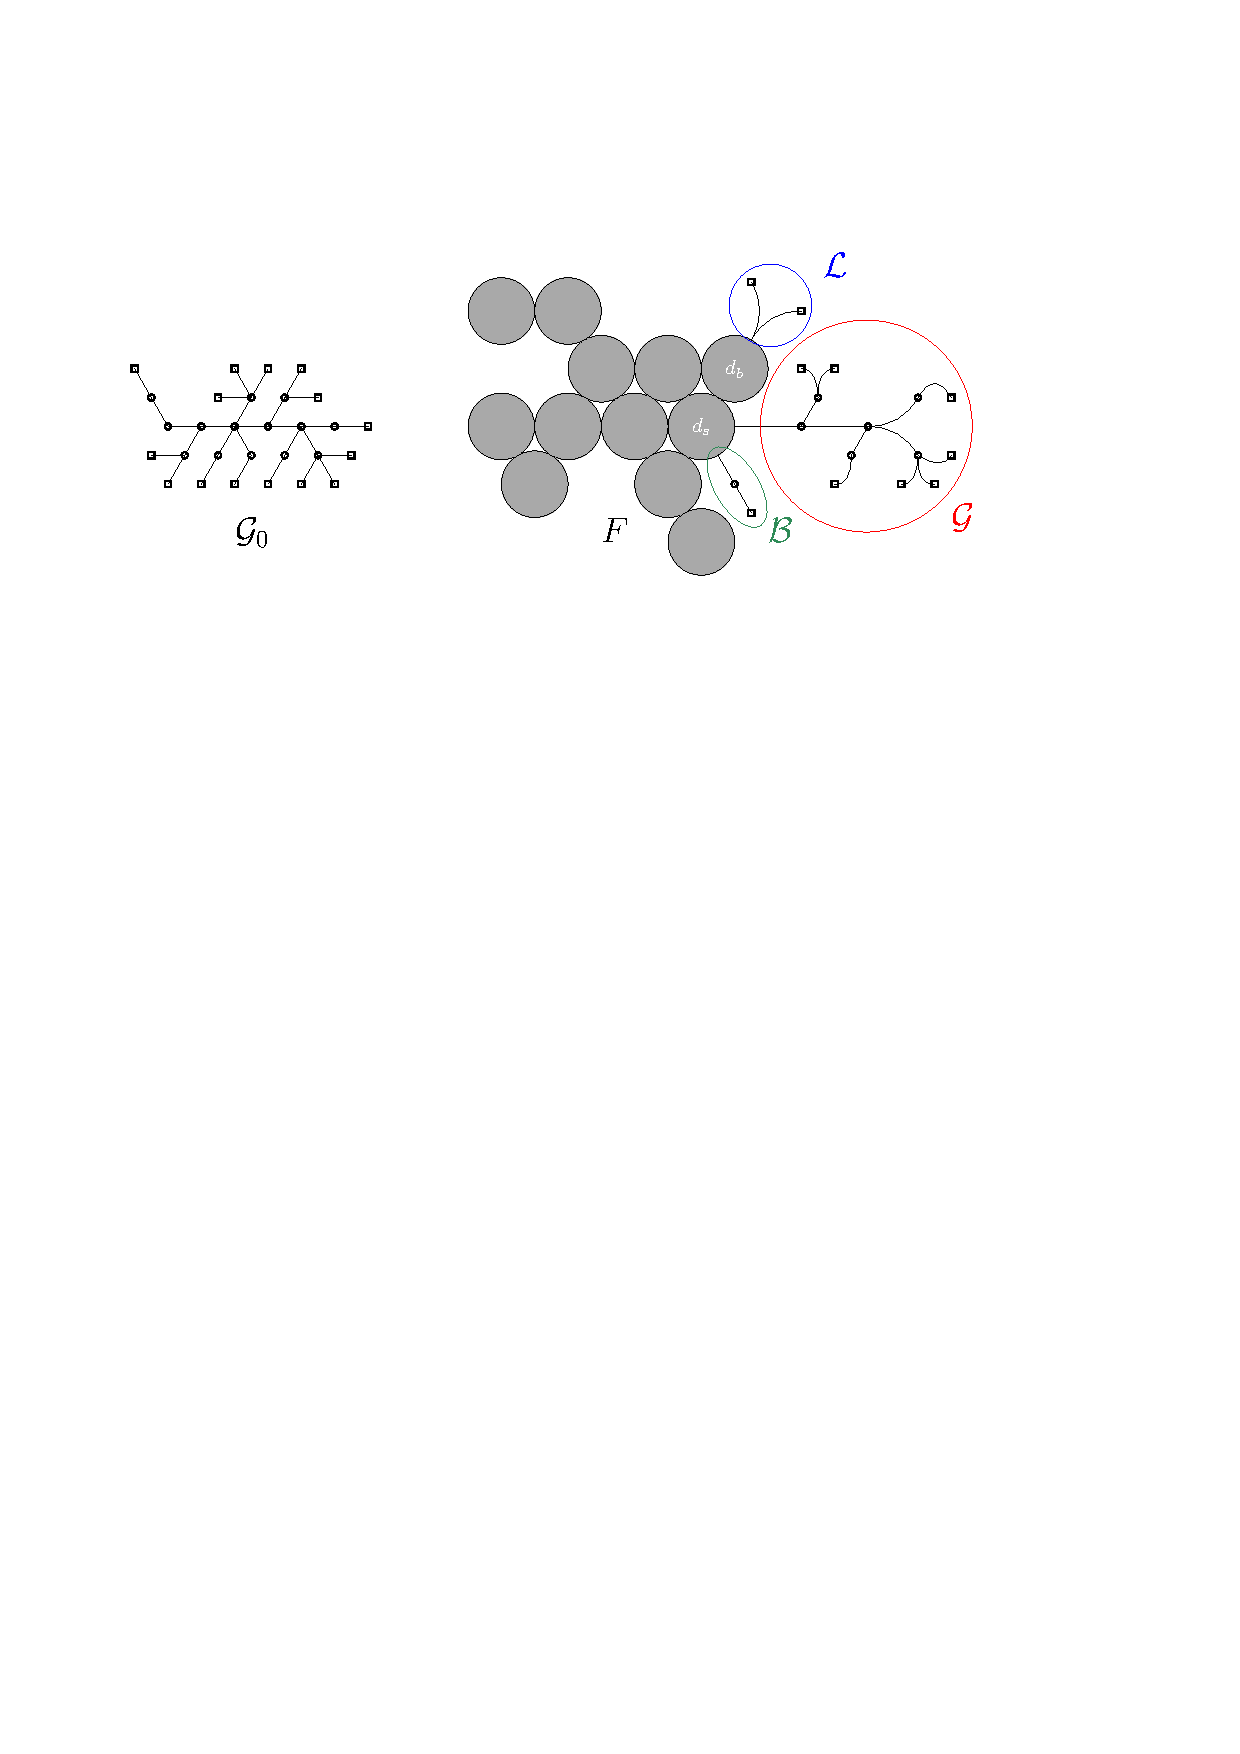
\includegraphics{graphics/dp-problem.pdf}
    \caption{Illustration of an instance of the partial embedding problem.}
    \label{fig:dp-problem}
\end{figure}

To elaborate:

\begin{itemize}
    \item The spine head $d_s$ and branch head $d_b$ are the most-recently placed spine and branch disks, respectively.
    \item If the set of loose leaves $\mathcal L$ is non-empty, $d_b$ is always adjacent to $d_s$.
    \item The \emph{order} $\leq_{\mathcal G_0}$ is constant over all descendant problem instances. At any point, all $d_\ell \in \mathcal L$ are ordered before $d_b \in \mathcal B$ before $d_p \in \mathcal G$, with near spine disks before far spine disks. This order ensures that we always consistently choose the next disk to embed.
    \item Given a particular \emph{initial lobster} $\mathcal G_0$, there exists a unique \emph{initial partial embedding problem} in which $S = \mathcal B = \mathcal L = \emptyset$, $\mathcal G = \mathcal G_0$ and $\leq_{\mathcal G_0}$ is deterministically defined based on $\mathcal G_0$.
\end{itemize}

\medskip

We construct the sub-instances of the partial embedding problem instance as follows:

\begin{enumerate}
    \item Let $d$ be the next disk to embed in order.
    \item If there is no place available on the grid for $d$, abort. The instance has no solution.
    \item Let $p$ be one of the possible ($\leq 5$) grid coordinates for embedding $d$.
    \item Construct the fundament of the new sub-instance $F' = F \cup p$.
    \item Remove $d$ from the partial input.
    \begin{itemize}
        \item If $d \in \mathcal L$, let $\mathcal L' = \mathcal L \setminus d$.
        \item If $d \in \mathcal B$, let $\mathcal B' = \mathcal B \setminus d$ and $\mathcal L' = \Gamma^+(d)$ (leaves on this branch). Let $d_b' = d$ be the new branch head.
        \item If $d \in \mathcal G$, let $\mathcal G' = \mathcal G \setminus \Gamma^*(d)$ (remove $d$ with all branches and leaves). Let $\mathcal B' = \Gamma^+(d)$ (branches on this spine). Let $d_s' = d$ be the new spine head.
    \end{itemize}
\end{enumerate}

\begin{figure}[h]
    \centering
    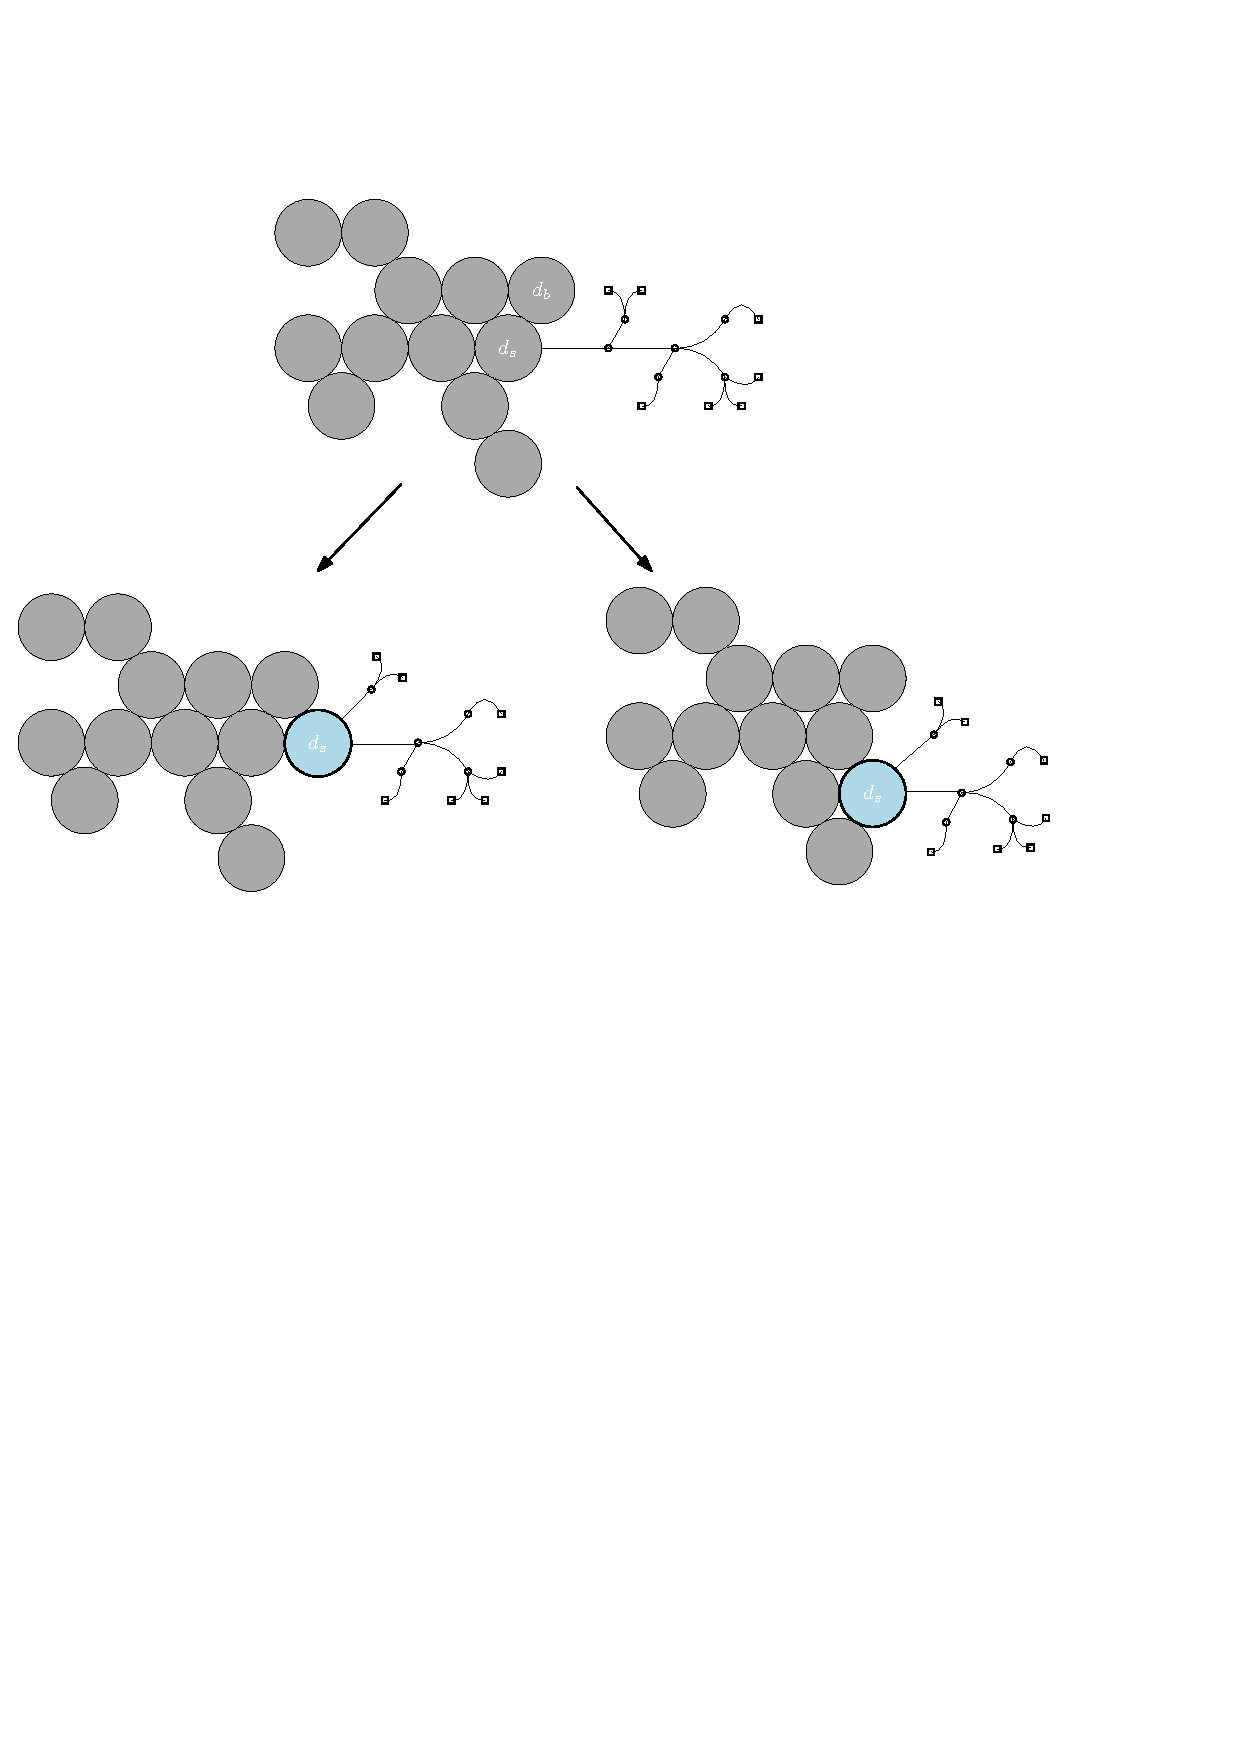
\includegraphics[width=\textwidth]{graphics/dp-subproblems.pdf}
    \caption{Sub-instances of an instance.}
    \label{fig:my_label}
\end{figure}

The solution to any of the thus constructed sub-instances is then also a solution to the whole \emph{partial embedding instance}.

\subsection{Instance Equivalence}

The limited branching factor and x-monotonicity property of lobsters ensure that the dynamic programming approach can theoretically find a solution in time linear in the size $n$ of the lobster.

However, to estimate real-world tractability, we must examine the number of concurrent partial embedding instances that can emerge in this approach.

This amounts to enumerating all the possible configurations of the \emph{local fundament}, which is restricted to the area where the \emph{fundament} may overlap and thus interfere with future disk placement.

(figure illustrating locality = fundament cap reach)

We generally consider or expand the partial instances in a breadth-first-search manner, that is, in order of increasing size of the fundament. The number of instances at any given size is bounded by a (large) constant. We can ``forget'' about partial instances once expanded, because their solution will be given in entirety by the solution of some descendant problem. Therefore the question of equivalence of two partial instances can also ignore the size aspect.

\begin{definition}[Comparability]
Two partial embedding problem instances are \emph{comparable} if they are same-sized and based on the same $\mathcal G_0$.
\end{definition}

This implies that the order $\leq_{\mathcal G_0}$ of two comparable instances is the same as well.
We are only ever interested in comparing comparable instances and will from here on assume by convention that, whenever we talk about two instances in the same context, that they are comparable.

This brings us to the key definitions for determining the worst-case cost of the dynamic programming approach.

\begin{definition}[Equivalence]
Let $\mathbf P_1$ and $\mathbf P_2$ be two comparable partial embedding problem instances. $\mathbf P_1$ and $\mathbf P_2$ are \emph{equivalent} if and only if for any embedding $\mathcal E(\mathcal G_0)$ that solves $\mathbf P_1$, we can construct a not necessarily different embedding $\mathcal E'(\mathcal G_0)$ that solves $\mathbf P_2$.
\end{definition}

\subsection{Towards an Upper Complexity Bound}

\begin{definition}[Breadth]
The \emph{breadth} $\overline{m}$ of the partial embedding problem is the maximum number of equivalence classes that may emerge among comparable problem instances.
\end{definition}

The breadth $\overline{m}$ is the above-mentioned ``number of concurrent partial embedding instances'' that we are interested in.
We now determine an upper bound for $\overline{m}$.

\begin{definition}[Reach]
The \emph{reach} $R(P)$ of the partial lobster $P$ is the set of possible grid coordinates where future disks may yet be embedded, disregarding the fundament.
\end{definition}

\begin{definition}[Local Fundament]
The \emph{local fundament} $F_L \subseteq F$ of a partial embedding instance is the subset of the fundament which intersects the reach area.
\end{definition}

The shape of the local fundament of an instance, relative to its spine head $d_s$ and together with its branch head $d_b$, determines the equivalence class of the instance.

This allows us to make a first attempt at an upper bound.

Since every grid coordinate $p$ in the worst-case (maximally reach-overlapping) local fundament can be occupied ($p \in F$) or not ($p \not\in F$), the breadth value may double accordingly.

Additionally, there are at most 6 possible positions of $d_b$.

(figure depicting worst-case fundament)

In formal terms:

\begin{equation}
    \overline m \leq 2^{\left\lvert \bigcup\limits_{\forall F_L \forall P} F_L \cap R(P) \right\rvert} * 6.
\end{equation}

Figure~\ref{} shows that the size of the area that we must consider under this approach is 24 coordinates. There are therefore less than $2^{24}*6$ concurrent instances.

\subsection{Refinement of the Upper Complexity Bound}

On closer consideration of the \emph{equivalence} definition above, there are many more instances with different fundaments which are also equivalent. We can improve our estimate of an upper bound by applying the following rules.

\begin{theorem}
Two comparable instances $\mathbf P_1$ and $\mathbf P_2$ are equivalent if the fundament and $d_b$ coordinate of $P_1$ is the mirrored fundament and $d_b$ coordinate of $P_2$.
\end{theorem}

\begin{theorem}
Two comparable instances $\mathbf P_1$ and $\mathbf P_2$ are equivalent if their fundament and $d_b$ coordinate can be matched by applying a rotation (around $d_s$).
\end{theorem}

\begin{theorem}
The $d_b$ coordinate is irrelevant to equivalence if the set of loose leaves $\mathcal L$ is empty.
\end{theorem}

\begin{theorem}
A grid coordinate $p \in F_L$ is irrelevant to equivalence if it is \emph{occluded}, i.e. not reachable from future disks in any scenario.
\end{theorem}

To be continued.

\section{Heuristic Approach}

We examine a fast approach to embed a lobster graph in linear time.
This algorithm is based on a small set of heuristics.
It is not guaranteed to find an embedding if one is possible.

The algorithm simply attempts to embed one node after the other into a triangular grid of coordinates.

\subsection{Embed Order}

Parent node are always placed before their children, where

\begin{itemize}
    \item the parent of every spine node is the previous spine,
    \item the parent of a branch is a spine and
    \item the parent of a leaf is a branch.
\end{itemize}

Beyond that, the heuristic algorithm can be configured with an ``order'' parameter, which is one of the following:

\begin{itemize}
    \item \emph{depth-first}: place all leaves on a branch before placing the next branch,
    \item \emph{breadth-first}: place all branches on the current spine node, then all their leaves.
\end{itemize}

(2 diagrams to illustrate)

When it decides on a location to embed a node, the algorithm considers all the adjacent coordinates to the parent node.
The spine is laid out in a line, initially from left to right.
When it appends branches or leaves, it leaves as much space as possible in the front for later nodes by preferring to embed them at locations at the back.

(diagram to illustrate preference for back)

\subsection{Space Heuristic}

The heuristic algorithm employs a ``space heuristic'', which applies when it embeds branch nodes.
For every candidate location for a node, it considers the number of empty slots in its immediate neighborhood. If there are not enough free locations to fit the known number of leaves on that branch, the location is disqualified and the algorithm moves on to the next candidate.

(diagram to illustrate space heuristic)

\subsection{Bend Heuristic}

The ``bend heuristic'' is applied to spine nodes.
Every spine node has a principal direction, which dictates the meaning of the \emph{relative} directions for its descendant nodes (like the ``back'' and ``front'' in the basic placement heuristic above).
The next spine node can be attached to its precursor in any of the six cardinal directions of the triangular grid. However, at every step, preference is given to the direction which leaves the most free space in its two-step vicinity.
If the nodes embedded so far lean ``heavy'' in one direction - above or below the spine - this allows us to introduce a \emph{bend} in the spine towards the direction that will hopefully allow us to place more branches and leaves later on.

(diagram to illustrate bend heuristic)

\section{Data Structures}

Both algorithms start with a caterpillar in \emph{degree list representation}.
This is a list of node degrees associated with the spine of the graph.
The degree of a spine vertex is the number of neighbor spine vertices (1--2) plus the number of attached leaves. Figure~\ref{fig:degree_repr} illustrates the concept.

\begin{figure}
    \centering
    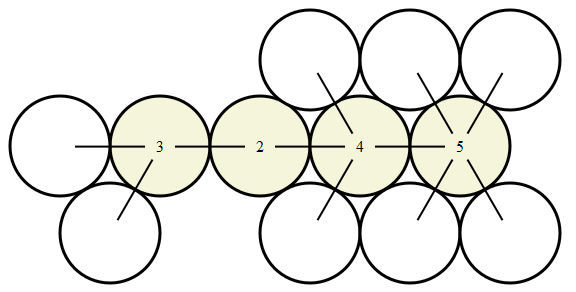
\includegraphics[width=240pt]{graphics/degree_repr.png}
    \caption{Embedding for the caterpillar with degree representation (3, 2, 4, 5).}
    \label{fig:degree_repr}
\end{figure}

If the input graph is supplied in one of the other formats understood by the program, it first converts the data into the internal representation. This is possible for any graph in linear time.
Since a caterpillar is ``a tree for which a path remains after removing all leaves'' \cite{Klemz2015}, the procedure is:

\begin{enumerate}
    \item Remove all leaves from the input.
    \item Locate the spine formed by the \emph{inner path} of the original graph --- look for any vertex with remaining degree of 1.
    \item Count the degrees of every path node in the original graph.
    \item Remember the original node identifiers of the spine vertices.
\end{enumerate}

The output data structure (Figure~\ref{fig:output_repr}) accounts for the desired graph layout as well as some practical considerations.

\begin{figure}
    \centering
    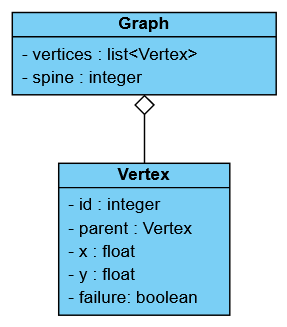
\includegraphics[width=180pt]{graphics/output_repr.png}
    \caption{Internal representation of the algorithm's output.}
    \label{fig:output_repr}
\end{figure}

\begin{itemize}
    \item The \texttt{id} attribute maps the vertex to its original identifier in the input graph.
    \item An association line is drawn in the output from the leaves to their \texttt{parent}s for illustration.
    \item The \texttt{failure} flag indicates vertices which could not be placed as described below.
\end{itemize}

\section{Weak Contact Representation}

All vertices in this method are aligned on a triangular grid.
Place the \emph{spine} $(v_0, \ldots , v_n)$ on the coordinates $(0,0), (1,0), \ldots , (n,0)$.

\begin{figure}
    \centering
    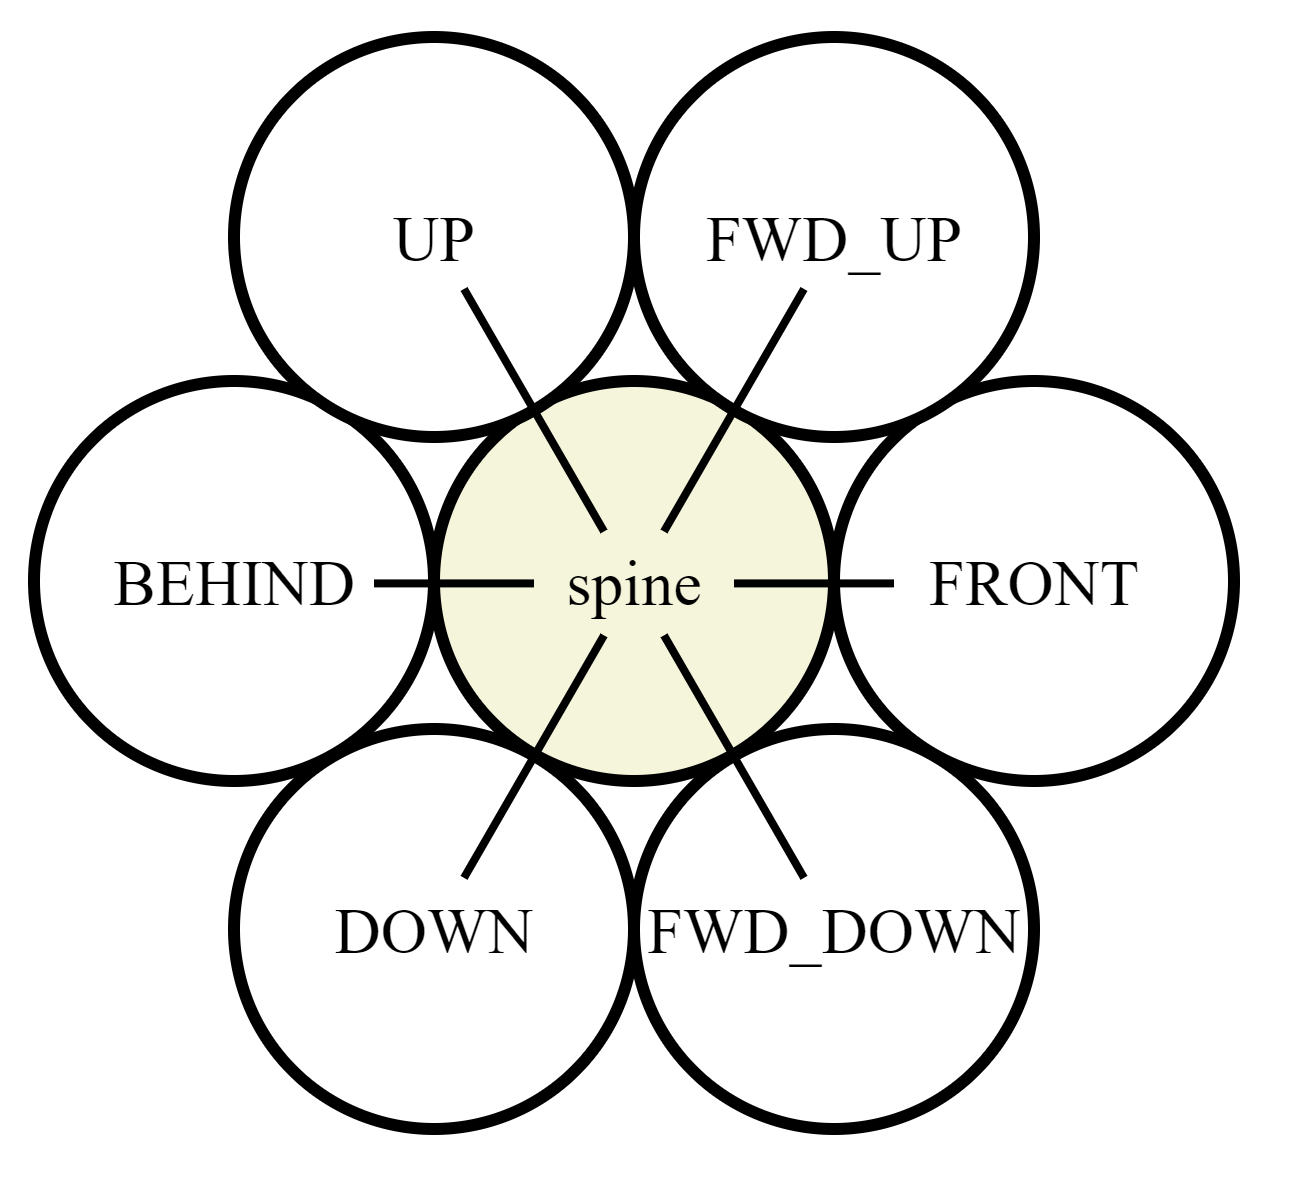
\includegraphics[width=180pt]{graphics/slots.png}
    \caption{Slot positions relative to the current spine vertex.}
    \label{fig:slots}
\end{figure}

For each spine vertex in order, assign leaves to the coordinates indicated by the next free \emph{slot}.
The slot is an ordinal type that can easily be maintained for each leaf placed and when advancing from one spine vertex to the next.
Figure~\ref{fig:slots} illustrates the available slots.

\section{Strict Contact Representation}

In this algorithm, the placement of spine vertices and leaves is based on a consideration of where there is space available to place them.
For each spine disk $(D_0, \ldots , D_{n-1})$, it places all the leaves of spine vertex $i-1$ before the disk $D_i$ itself.

The placement of any vertices is generally directed by the concept of the

\begin{quote}
``bisector of the free space, which we define as the maximum cone with origin in $D_{i-1}$'s center containing no previously inserted neighbors of $D_{i-1}$ or $D_{i-2}$.'' \cite{Klemz2015}.
\end{quote}

Spine vertices are placed in the center of this bisector, while leaves are alternatingly placed as far up and as far down as possible.
The placement of a leaf disk is therefore constrained by the following factors:

\begin{itemize}
    \item The distance to the current spine disk must be $1$ to implement unit disk contact.
    \item It must not be placed so far back as to intersect the previous spine vertex.
    \item It must not intersect the previous leaf disk on the same side either.
    \item The distance to other disks without contact must consider the \emph{gap} parameter.
\end{itemize}

The \emph{gap} is an additional feature which extends the original algorithm to provide a visual distinction between disks in contact and disks not in contact with each other. It is available as a configuration parameter to the user of the program.

\begin{figure}
    \centering
    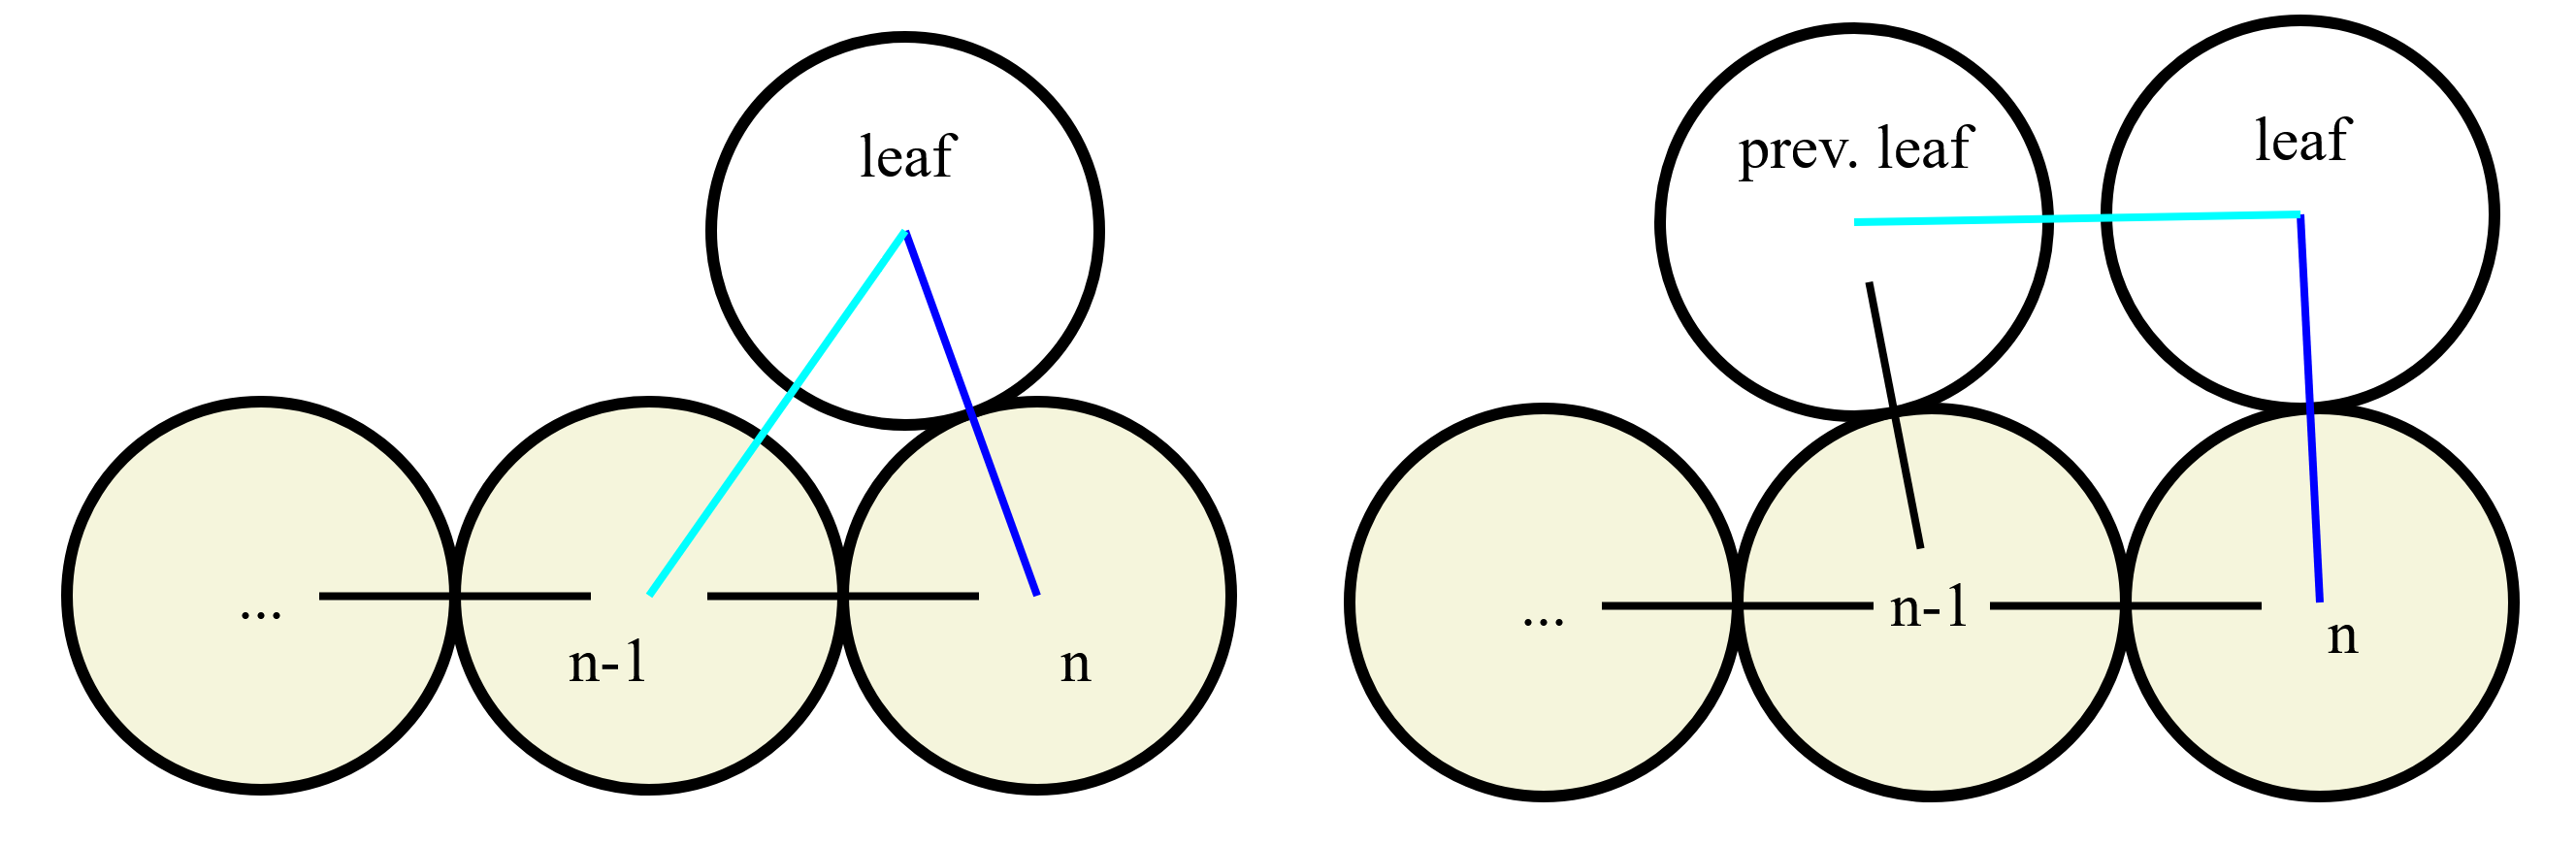
\includegraphics[width=\textwidth]{graphics/strict_contact.png}
    \caption{Constraints in placement of the next leaf vertex.}
    \label{fig:strict_contact}
\end{figure}

Figure~\ref{fig:strict_contact} illustrates the placement constraints for disks in the strict contact representation algorithm. The blue line of unit length shows the distance to the leaf in contact with the associated spine vertex. The cyan line is the distance from the nearby constraining vertex. Its length is $1 + gap$.

\section{Visualizing Failure}

A disk contact representation exists only for caterpillars which satisfy the constraints on the number of leaves as proven by Cleve \cite{Cleve2020}, Klemz, Nöllenburg and Prutkin \cite{Klemz2015}.

The \texttt{udcrgen} program will accept as input and create embeddings for ``overflowing'' caterpillars with too many leaf vertices.
It places excess vertices at separate coordinates which do not conform to the disk contact rules and sets them apart with a highlight color as shown later in Figure~\ref{fig:failure}. This shows the user \emph{why} an excessive caterpillar cannot be embedded with unit disk contact.

\section{Performance Measurement}

Cleve \cite{Cleve2020}, Klemz, Nöllenburg and Prutkin \cite{Klemz2015} have shown that both weak and strict contact representations can be decided (and calculated) for caterpillars in linear time. This work corroborates this result empirically with run-time performance measurements of the implemented algorithms on a benchmark set of input graphs.

The benchmark was run on a machine with a consumer-grade Intel Core i5-1035G4@1.10GHz CPU.

% Remove following line for the final thesis.
%\input{intro.tex} % A short introduction to LaTeX.

\chapter{Evaluation}

\section{Visual Comparison}

The program produces images that resemble the reference images. See Figure~\ref{fig:visual_comparison}, with the illustrations by Cleve \cite{Cleve2020} (top left) and Klemz et al. \cite{Klemz2015} (bottom left), which the authors embedded manually. Compare them with the corresponding \texttt{udcrgen} output on the right. 

\begin{figure}
    \centering
    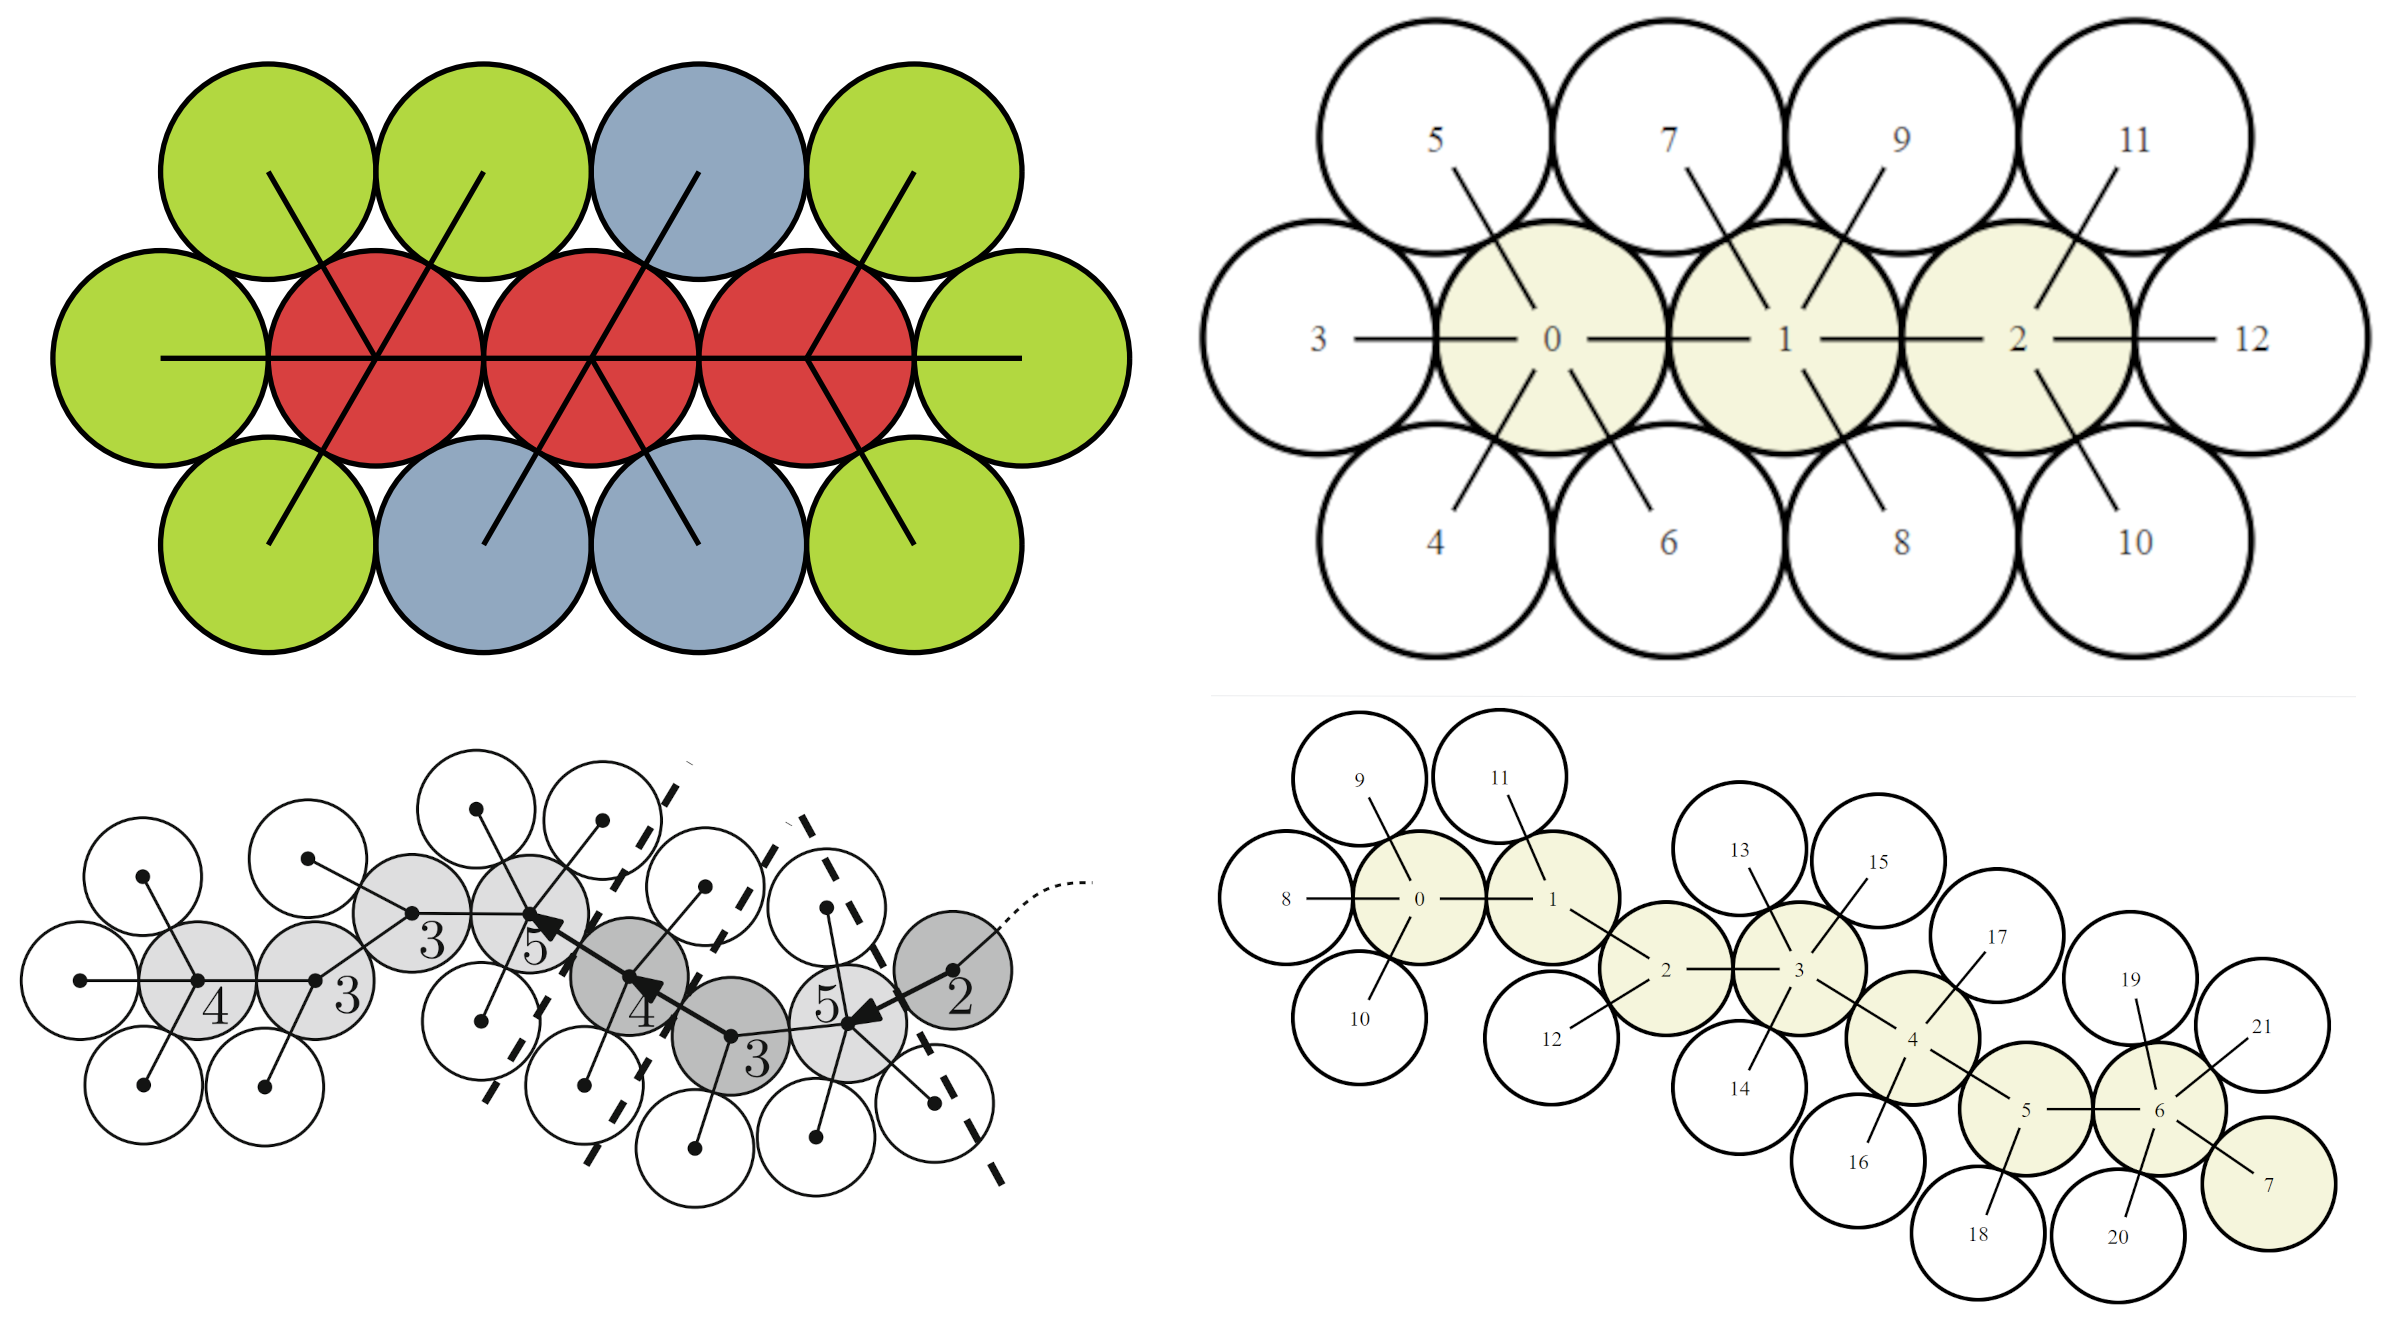
\includegraphics[width=\textwidth]{graphics/visual_comparison.png}
    \caption{Original papers vs \texttt{udcrgen} output.}
    \label{fig:visual_comparison}
\end{figure}

\section{Failure Output}

Figure~\ref{fig:failure} shows how the program visualizes embedding failures for excessive inputs with highlights.

\begin{figure}
    \centering
    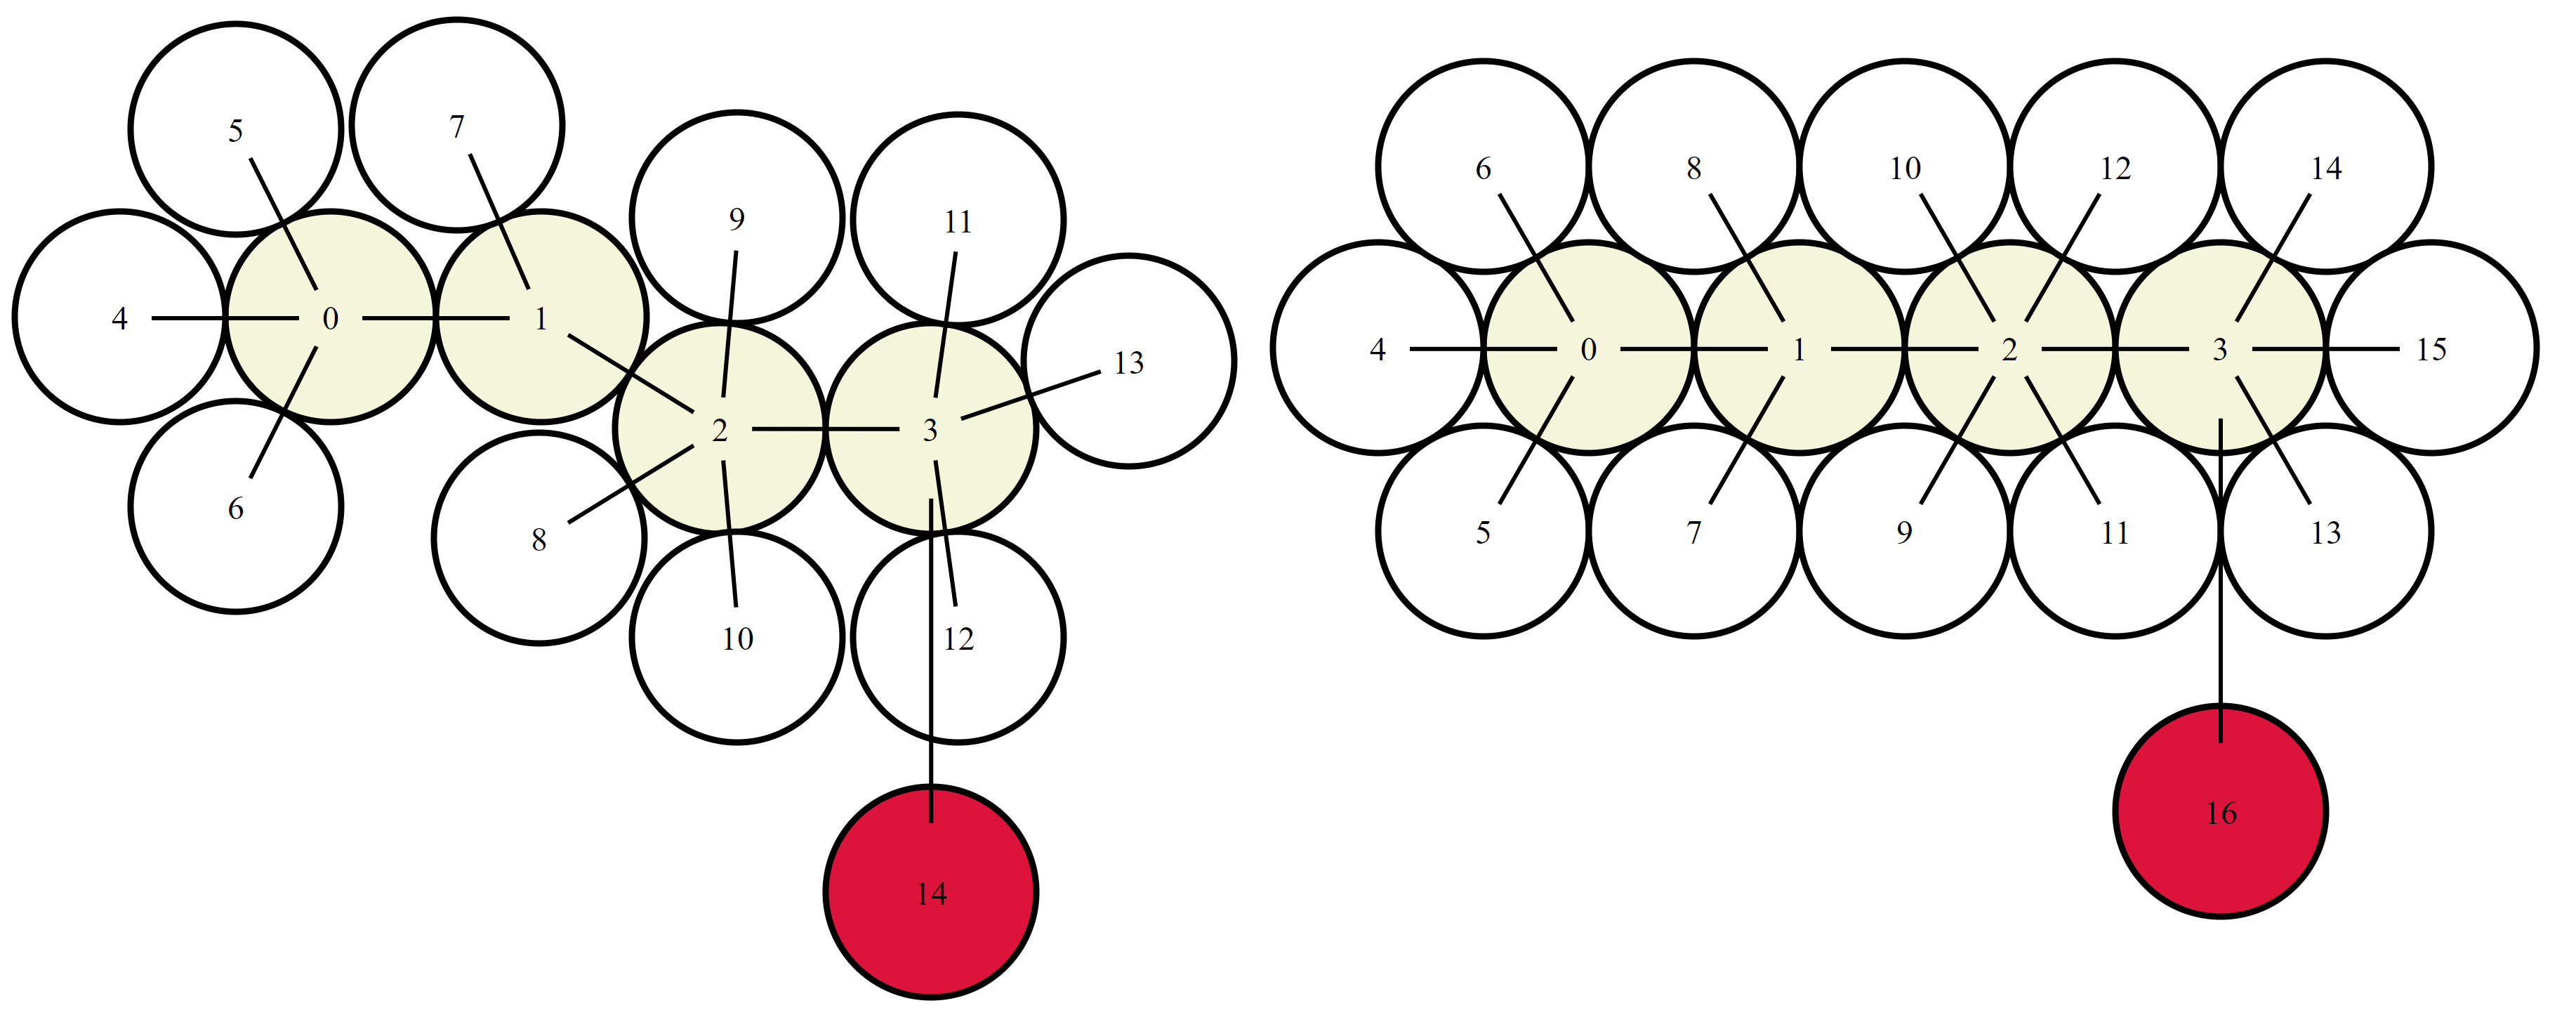
\includegraphics[width=\textwidth]{graphics/failure.png}
    \caption{Caterpillars without unit disk contact embedding, illustrated.}
    \label{fig:failure}
\end{figure}

\section{Run Time Measurements}

% \begin{table}[t]
%     \centering
%     \caption{Run time to generate an embedding for a caterpillar.}
%     \label{tab:runtime_performance}
%     \begin{tabular}{lll}
%         \toprule
%         spine length & time (weak contact) {[}ms{]} & time (strict contact) {[}ms{]} \\
%         \midrule
%         100          & -                     & -                       \\
%         500          & -                     & -                       \\
%         1000         & -                     & -                       \\
%         2000         & -                     & -                       \\
%         5000         & -                     & -                       \\
%         10000        & -                     & -                       \\
%         \bottomrule
%     \end{tabular}
% \end{table}

% Table~\ref{tab:runtime_performance} shows the run times that were observed on the benchmark inputs. Refer to Figure~\ref{fig:runtime_plot} for a visual plot.
These results are consistent with our expectation of linear run time.

% \begin{figure}
%     \begin{tikzpicture}
%     \begin{axis}[
%         xlabel={spine length},
%         ylabel={time (weak embedding) {[}ms{]}},
%         xmin=0, xmax=10000,
%         ymin=0, ymax=3000,
%         xtick={0,2000,4000,6000,8000,10000},
%         ytick={0,500,1000,1500,2000,2500,3000},
%         legend pos=north west,
%         ymajorgrids=true,
%         grid style=dashed,
%     ]
    
%     \addplot[
%         color=blue,
%         mark=square,
%         ]
%         coordinates {
%         (100,24)(500,102)(1000,244)(2000,483)(5000,1210)(10000,2441)
%         };
        
%     \addplot[
%         color=red,
%         mark=square,
%         ]
%         coordinates {
%         (100,30)(500,148)(1000,291)(2000,612)(5000,1499)(10000,2967)
%         };
        
%         \legend{weak contact, strict contact}
        
%     \end{axis}
%     \end{tikzpicture}
%     \centering
%     \caption{Plot of algorithm run time performance.}
%     \label{fig:runtime_plot}
% \end{figure}

\backmatter

% Use an optional list of figures.
% \listoffigures % Starred version, i.e., \listoffigures*, removes the toc entry.

% Use an optional list of tables.
% \cleardoublepage % Start list of tables on the next empty right hand page.
% \listoftables % Starred version, i.e., \listoftables*, removes the toc entry.

% Use an optional list of alogrithms.
% \listofalgorithms
% \addcontentsline{toc}{chapter}{List of Algorithms}

% Add an index.
% \printindex

% Add a glossary.
% \printglossaries

% Add a bibliography.
\bibliographystyle{alpha}
\bibliography{bsc_thesis}

\end{document}